\documentclass[a4paper]{article}

\title{Lecture 2: Seqences, Limits and Infinites}
\author{Shashank Vatedka}

\usepackage{basicreq}
\usepackage{./teaching_doc_macros}
\DeclareMathOperator*{\maxi}{Max}
%\DeclareMathOperator*{\lim}{Lim}
\begin{document}

%FILL IN THE RIGHT INFO.
%\lecture{**LECTURE-NUMBER**}{**UNIT**}{**LECTURER**}{**SCRIBE**}
\lecture{2}{SEQUENCES, LIMITS AND INFINITES}{Shashank Vatedka}{EE20RESCH14005}
%\footnotetext{These notes are partially based on those of Nigel Mansell.}

% **** YOUR NOTES GO HERE:
\section{GIST OF LECTURE 1}
In the last lecture, we have seen the introduction topics such as\\
\begin{enumerate}
\item	What does a general communication system look like?
\begin{figure}[!ht]
\centering
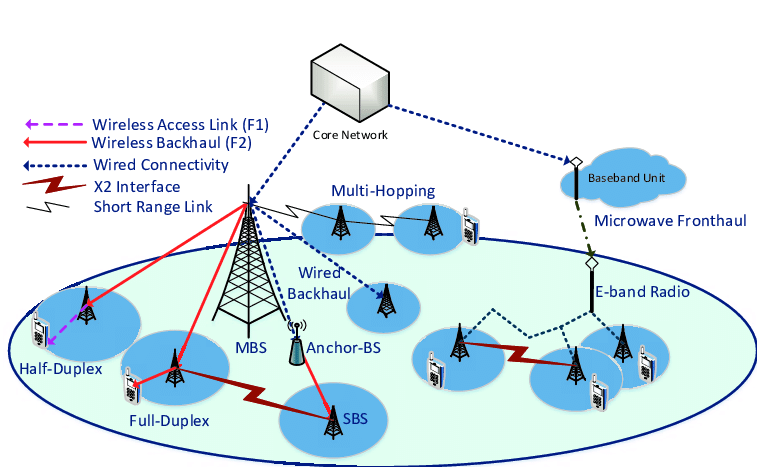
\includegraphics[width=6.0cm]{wireless image 1.png}
\caption{General Communication Systems}\label{fig:1}
\end{figure} \\
A general communication system consists of user equipments(source nodes) connected to base stations through wireless links otherwise called channels which are noisy. These base stations are inturn connected to a back haul network which connects to a core network via a wired/ optical link. They are to support a large number of users.\\
\\
In such systems, primary goal will be designing a noise free communication system which require modelling of source as well as channel. 
\\
\item \textbf{Single User/ Point-to-Point System}.\\
\begin{figure}[!ht]
\centering
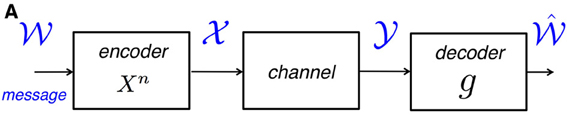
\includegraphics[width=6.0cm]{simple_encoder_decoder.png}
\caption{Single User/ Point-to-Point System}\label{fig:2}
\end{figure} \\
In a point-to-point/ single user communication system which is shown in above figure, the rate at which the communication may take place is given by
\begin{align}
\begin{split}
	\Rightarrow R = \frac{k}{n}
\end{split}
\end{align}
where k is number of useful message bits taken by encoder and generate codewords of n bits length.It may appear very simple. To measure the performance of the system, Rate(code rate) and $P_e$(bit error rate) are used. The discrete memoryless channel is defined by the transition probability matrix i.e. $P_{(Y|X)}$. The capacity of the channel is given by\\
\\
\begin{align}
\begin{split}
C=\maxi_{\mathbf{P_X}} I(X;Y)\\
\end{split}
\end{align}
\\
From Shannon Channel Coding Theorem, it is possible to design codes such that
\\
\\
\begin{align}
\begin{split}
\lim_{n \to \infty} R \approx I(X;Y)\\
\lim_{n \to \infty} P_e \approx 0\\
\end{split}
\end{align}
\\
\item \textbf{Multi-User Systems}.\\
\begin{figure}[!ht]
\centering
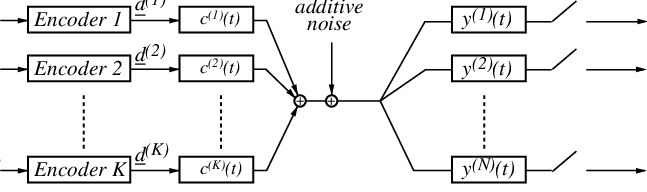
\includegraphics[width=6.0cm]{multi-user-systems.png}
\caption{Multi-User System}\label{fig:3}
\end{figure} \\
\\
In Multi-User Systems, goal is to receive the distinct number of messages without any loss or interference within the power constraints. The rate of transmission are given as below.
\\
\\
\begin{align}
\begin{split}
	\Rightarrow R_1 = \frac{k_1}{n}\\
	\Rightarrow R_2 = \frac{k_2}{n}...\\
\end{split}
\end{align}
\begin{enumerate}
\item How to mitigate effects of Interference?\\
By using a type of scheduling mechanism, one can avoid the interference caused by multiple signals generated by multiple users such as TDMA(most commonly used), FDMA etc.,.
\\
\item How to measure performance?\\
Consider only 2 users are trying to communicate using a system. Here assume the noise is Gaussian i.e. $W_i \sim \mathcal{N}(\mu = 0,\,\sigma^{2})$
In an AWGN channel, the max rate  is  given by
\begin{align}
\begin{split}
R_{max} = C = \frac{1}{2}*\log_2(1+\frac{P}{\sigma^2})\\
\text{where} \frac{P}{\sigma^2} = SNR.
\end{split}
\end{align}
\\
When any scheduling is done, the max rate is dependent on the time allotted or divided between the users. The max rates as per the user is given as below:
\begin{align}
\begin{split}
	\Rightarrow R_1 \leq \alpha C\\
	\Rightarrow R_2 \leq (1-\alpha C)\\
	where C = \frac{1}{2}*log_2(1+\frac{P}{\sigma^2})\\
\end{split}
\end{align}
If the plot of above rates is carried out, it will look below:
\begin{figure}[!ht]
\centering
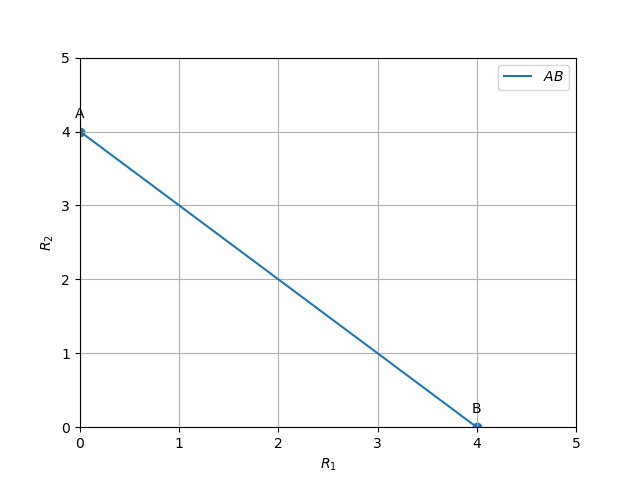
\includegraphics[width=6.0cm]{R1_R2.png}
\caption{Rate Performance Graph}\label{fig:4}
\end{figure} \\
\end{enumerate}
\item This performance is obtained by simply following simple TDMA techniques. Can we do better?
\\
The answer is Yes. The rate performance in a multi-user system can be improved by using a procedure called Successive Interference Cancellation(\textbf{SIC}). In this interference caused by another user is treated as noise and the rate of user 1 is calculated. First decode message of user 1 treating the codeword of user 2 as noise. Then remove the effect of the decoded codeword of user 1 from received signal and decode message of user 2. The rates can be obtained as below:\\
\\
\\
\\

\begin{align}
\begin{split}
	\Rightarrow R_1 = C = \frac{1}{2}*log_2(1+\frac{P}{P+\sigma^2})\\
	\Rightarrow R_2 = \frac{1}{2}*log_2(1+\frac{P}{\sigma^2})\\
\end{split}
\end{align}
\\
\\
\\

The plot of $R_1$ vs $R_2$ is shown below:
\begin{figure}[!ht]
\centering
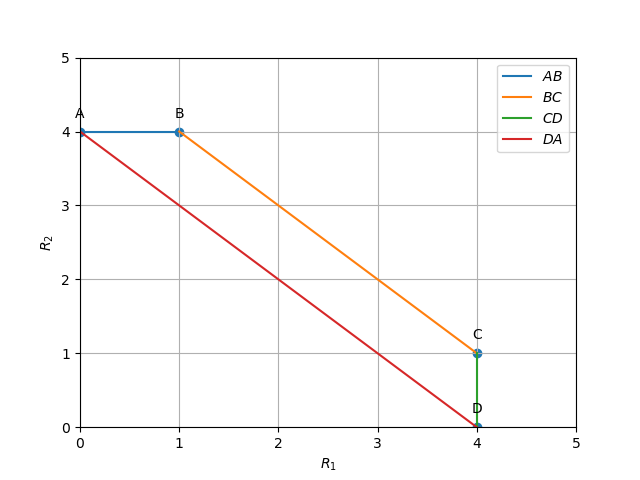
\includegraphics[width=6.0cm]{R1_R2_better.png}
\caption{Rate Performance Graph through SIC}\label{fig:5}
\end{figure} \\
\\There are more techniques which will further enhance of multi-user systems which will be studied in this course.
\end{enumerate}
\bigskip
\section{Sequences}
\subsection{Commonly used notations}
\begin{enumerate}
\item \textbf{R} - Rate
\item $P_e$ - Probability of Error
\item X, Y, Z...  - Random Varaibles
\item x,y,z..... - Deterministic Variables
\item $\bR$ - Real Numbers, $\bZ$ - Integers, $\bN$ - Natural numbers
\item Pr[X=x] - Probability Distributive Function
\item $P_x$ - Probability Mass Function (pmf)
\item $f_x$ - Probability Density Function (pdf)
\item $P_{(x|y)}(X|Y)$ - Conditional pmf
\item $f_{(x|y)}(X|Y)$ - Conditional pdf
\end{enumerate}
\subsection{Sequences}

As we have seen earlier, the design considerations are
\begin{align}
\begin{split}
\lim_{n \to \infty} R \approx C
\\
\lim_{n \to \infty} P_e \approx 0
\end{split}
\end{align}
i.e As the users increase, the rate at which they communicate should be as close as to capacity of channel and their communication should be error free and noise free with almost 0 probability of error.\\
\\
In Information Theory, one has to deal with huge number of users, limits, Channels and their time limits. A lot of mathematics is involved and they have to be exercised vary carefully. Above are some commonly used notions to understand the further notes.Let us understand mathematics involved. Since Information Theory deal with a lot of sequential data and process, lets start with definition of sequence.
\\
\\
\textbf{Definition of a Sequence.}
\\
\\
\textbf{Informally}: A sequence is a ordered collection of numbers. These numbers may belong to sets of Natural($\bN$) or Integer($\bZ$) or Real numbers ($\bR$).\\
\\
\textbf{Formally}: A sequence over $\cA$ is defined as a function that maps any type of integer or number from the set of Natural($\bN$) to set $\cA$ i.e. $f:\bN \to \cA. \cA$ can be any set. \\
\\
\textbf{Example-1:}
\\
Let $\cA = {1,\frac{1}{2},\frac{1}{3},\frac{1}{4},....}$.
Here the set $\cA \subset \bR$. The numbers follow a pattern and it can be represented by a funtion and it is $f = \frac{1}{n}$. So a sequence typically have a function which maps numbers from set $\bR$ to its subset.\\
\textbf{Example-2:}
\\
Let $\cB = {1,\frac{1}{2},\frac{1}{4},\frac{1}{8},....}$.
Here the set $\cB \subset \bR$. The numbers follow a pattern and it can be represented by a function and it is $f = 2^{-(n+1)}$. 
\\
\\
Q) Are these sequences finite or infinite ?
\\
They are infinite in nature.As an exmaple, lets consider sequence defined by $f=\frac{1}{n}$. It is continuously increasing(in denominator) till infinity. Here the concept of limits will restrict the increment or decrement of sequence.
\\
\\
Q) Does every sequence have a limit ?\\
Based on the value of function,  every sequence may or may not have a limit. The one which limits to a finite value upon n incrementing to $\infty$ is called a convergent sequence. The one which does not limit to a finite value or if the function value is either $\infty$ or $-\infty$ then it is called as Divergent Sequence. To denote the limit, it is written as
\\
\begin{align}
\begin{split}
\lim_{n \to \infty} f= \lim_{n \to \infty} \frac{1}{n} = \frac{1}{\infty} = 0
\end{split}
\end{align}
\\
\\
In the above example of $f=\frac{1}{n}$, as n $\to -\infty\  \text{or}\  \infty$ the value of f will be 0 i.e. the sequence converges to 0. If $f={n}$, then as n $\to -\infty\  \text{or}\  \infty$ the value of f will be $\infty$ and the sequence does not converge to finite value. Hence it is a divergent sequence. 
\\
\\
\textbf{Bounded Sequences.}
\\
\\
If any sequence contains a number of elements less than a particular value or number i.e. limit then the sequence is called a Bounded sequence. Else it is unbounded sequence. Limits are well elaborated in next section. \\
Formally, consider M, a real number and $M\geq0$. A finite sequence $a_1,a_2,a_3,....a_n$ for a finite n is bounded by M iff $\mid a_i \mid \leq M , \forall 1 \leq i \leq n$. 
 An infinite sequence $(a_n)^{\infty}_{n=1}$ i.e.$a_1,a_2,a_3,....a_\infty$ is bounded by M iff $\mid a_i \mid \leq M , \forall i \geq 1$. \\
 \\
Combinedly, a sequence is said to be bounded iff it is bounded for some rational number M $\geq$ 0.
\\
\\
\textbf{Example-3}.A sequence by function $f=(-1)^n i.e. for n=0, 1 ,2,3,4,...\infty$ the sequence can be written as $1,-1,1,-1,1,-1,1,-1,...$ respectively. Consider M $>$ 1, and for any value of n, $\mid a_i \mid \leq M $. Hence it is a bounded sequence.
\\
\\
\textbf{Example-4}.A sequence by function $f=2^{-n} i.e. for n=0, 1 ,2,3,4,...\infty$ the sequence can be written as $1,\frac{1}{2},\frac{1}{4},\frac{1}{8},......2^{-\infty}$ respectively. Consider M $\geq 1$, $\mid a_i \mid \leq M $. Hence it is a bounded sequence.
\\
\\
\textbf{Example-5}.A sequence by function $f=-n^2 i.e. for n=0, 1 ,2,3,4,...\infty$ the sequence is $0,-1,-4,-6,-9...-\infty$ respectively. , and for any value of M, $\mid a_i \mid \geq M $. Hence it is a unbounded sequence. 
\\
\\
\textbf{Note}. Every finite sequence is a bounded sequence. For a rational sequence, such as $f=\pi$ for a finite n in decimal places, f will be a finite rational number and limit to it. As $n \to \infty$, f(n) will limit to a irrational number. Here the limits have to well-defined. Hence the concept Supremum and Infimum of a set.
\\
\\
\textbf{Open and Closed Sets}.
\\
\\
Bounds of a function are defined in the form of a set/range i.e (lower bound, upper bound). Any sequence will lie within the specified bounds. The type of braces/brackets used defines the closedness of a set. For $f=\frac{1}{n+1}$ i.e. sequence $\frac{1}{2},\frac{1}{3},\frac{1}{4},....$ f(n) $\to$ 0. The sequence is defined over set $\cA$ = (0,1). Here the sequence converges to 0 and it is not included in the set (0,1). Here $\cA$ is called open set. By definition, \textbf{Open set} is a set in which the set of lower bound and set of upper bound does not form subset of the set i.e. for the above set $\cA$, lower limit is 0 and upper limit is 1. ${[0]},{[1]} \nsubseteq \cA$. If they form the subsets i.e. ${[0]},{[1]} \subseteq \cA$ then the set is called \textbf{Closed set} and the set is represented by using square brackets (a mathematical notation to define the closed set) i.e. $\cA$ = [0,1].
\\
\\
\textbf{Supremum}.
\\
\\
Supremum is defined as the least upper bound that is greater than any other number in the set. Let $\cA \subset \bR$.a is the supremum of $\cA$ iff\\
\begin{align}
\begin{split}
a \geq x,\quad \forall x \in \cA\\
or\\
\forall \epsilon \geq 0,\quad \exists x \in \cA 
\\such \ that \quad x > a-\epsilon \quad or \quad a < x+\epsilon
\end{split}
\end{align}
\\
\\
\textbf{Infimum}.
\\
\\
Infimum is defined as the greatest lower bound that is lesser than any other number in the set. Let $\cA \subset \bR$ and b is the infimum of $\cA$ iff\\
\begin{align}
\begin{split}
b \leq x, \quad \forall x \in \cA\\
or\\
\forall \epsilon \geq 0,\quad \exists x \in \cA 
\\such\  that \quad x > b+\epsilon \quad or \quad b < x-\epsilon
\end{split}
\end{align}
\\
\\
It is also to be noted that sequences may converge to a point either inside or outside the set. Hence it is not necessary that both supremum and infimum lie within the set. For an open set, they lie outside the set.
\\
\textbf{Example-6}:
\\
\\
Let $\cA$=(0,1) be an open set. Supremum for this set can be 1 and infimum be 0.Here if x=0.99991, x $\in \cA$, but $0, 1 \notin \cA$. 
\\
\\
It is to be noted that for a closed set, Supremum and Infimum lies within the set.\\
Supremum = max value of the set \\ Infimum = min value of the set. 
\\
\\
\textbf{Example-7}:
\\
\\
Let $\cA =(-2)^{n}:n\in \bZ$ be a sequence and is defined over a closed set $[-\infty,\infty]$. 
\begin{align}
\begin{split}
\Rightarrow Sup\ \cA = \infty\\
\& Inf\ \cA = -\infty.
\end{split}
\end{align} 
\\
\\
\subsection{Limits of Sequences}.

Though the bounds define the nature of sequence to an extent, their nature will be more evident from the limits of that sequence. The limit of a sequence is defined as the value to which a sequence $(a_n)^{\infty}_{n=m}$  converges to, for any value m and m $< \infty$. Let L be a rational number to which the sequence converges to, then the limit is written as\\
\begin{align}
\begin{split}
L \ = \ \lim_{n \to \infty} (a_n)
\end{split}
\end{align}
\\
\\
Distance between any two real numbers a and b is given by d(a,b) = $\mid a-b \mid$.\\
\\
Limit in terms of distance:
\\
For a function f: $\bN \to \cA$, with a constant difference of d in sequence i.e.($\cA$,d), if $(f_n)_{n\geq1}$ is a sequence over $\cA$ and $f_n \ converges \to a$ then\\
\begin{align}
\begin{split}
\Rightarrow \lim_{n \to \infty} f_n = a\ if\ \forall \epsilon > 0, \exists\ m\in \bN\ such\ that\ d(f_n, a) \leq \epsilon,\ \forall n\geq m
\end{split}
\end{align}

In \textbf{Example-3}, a sequence by function $f=(-1)^n i.e. for\ n=0, 1 ,2,3,4,...\infty$ is given. The sequence is $1,-1,1,-1,1,-1,1,-1,...$ respectively. $\forall M > 1$, and for any value of n, $\mid a_i \mid \leq M $. Hence it is a bounded sequence.The limits of n are given as n $\to -\infty\ or\ \infty$, the value of the sequence will be equal -1 or 1 as n $\to \infty$ or $-\infty$. Hence the sequence is not convergent but bounded sequence
\begin{align}
\begin{split}
\Rightarrow \lim_{n \to \infty} (-1)^n = either \  1 \ or\ -1.\\
\Rightarrow \lim_{n \to -\infty} (-1)^n = either \  1 \ or\ -1.
\\
\end{split}
\end{align}
\\
\\
In \textbf{Example-4}, a sequence by function $f=2^{-n} i.e. for\ n=0, 1 ,2,3,4,...\infty$ is written as $1,\frac{1}{2},\frac{1}{4},\frac{1}{8},......2^{-\infty}$ for respective n. $\forall$M $\geq 1$, $\mid a_i \mid \leq M $. Hence it is a bounded sequence.The limits of n are given as n $\to -\infty\ or\ \infty$, the value of sequence to which it converges to is 0. 
\begin{align}
\begin{split}
\Rightarrow \lim_{n \to \infty} 2^{-n} = 0.\\
\Rightarrow \lim_{n \to -\infty} 2^{-n} = 0.
\\
\end{split}
\end{align}
Hence it is convergent bounded sequence.
\\
\\
In \textbf{Example-5},a sequence by function $f=-(n^2) i.e. for\ n=0, 1 ,2,3,4,...\infty$ is written as $0,-1,-4,-6,-9...-\infty$ respectively, and for any value of M, $\mid a_i \mid \geq M $. Hence it is a unbounded sequence. Here, the limits of n are given as n $\to -\infty\ or\ \infty$, the value of sequence will $\to$ $-\infty$ and
\begin{align}
\begin{split}
\Rightarrow \lim_{n \to \infty} -(n^2) = -\infty.\\
\Rightarrow \lim_{n \to -\infty} -(n^2) = \infty.
\\
\end{split}
\end{align}
Hence it is a divergent unbounded sequence.
\\
\\
\textbf{Example-8}. For f(n) = $2^{-n}$.\\
\begin{align}
\begin{split}
\lim_{n \to \infty}2^{-n} = 0.\\
\Rightarrow \epsilon > 0, \exists m \ such\ that\ \mid 2^{-n}-0 \mid \leq\ \epsilon\\
\Rightarrow 2^{-n} \leq \epsilon\\
\Rightarrow n \geq log_2\frac{1}{\epsilon}\\
\Rightarrow for\ n \geq log_2\frac{1}{\epsilon}, \mid f(n)-0\leq \epsilon \mid.
\end{split}
\end{align}
\\
\\
\textbf{Example-9}. For f(n) = $log_2(1+\frac{3}{n})$.\\
\begin{align}
\begin{split}
\lim_{n \to \infty} log_2(1+\frac{3}{n})= 0.\\
\Rightarrow log_2(1+\frac{3}{n})\leq\epsilon\\
\Rightarrow 1+\frac{3}{n} \leq 2^\epsilon\\
\Rightarrow \frac{3}{n} \leq 2^\epsilon - 1 \\
\Rightarrow n \geq \frac{3}{2^\epsilon -1}\\
\Rightarrow for\ n \geq \frac{3}{2^\epsilon -1}, \mid f(n)-0 \mid \leq \epsilon.
\end{split}
\end{align}
\\
\\
\textbf{Note}: Limits are also called as limit points.
\\
\\
\textbf{Limit Superior}.
For any sequence $(a_n)^\infty_{n=m}$, define a new sequence $(a_N^+)^\infty_{N=m}$ using the supremum of  $(a_n)^\infty_{n=N} \Rightarrow a_N^+ = sup (a_n)^\infty_{n=N}$ and $a_N^+$ is the supremum of all elements in the sequence from $a_N$ onwards. The limit superior of $(a_n)^\infty_{n=m}$ is defined as 
	\\
	\\
	\begin{align}
	\begin{split}
	\lim\text{sup}_{n \to \infty} a_n = \lim_{n \to \infty} sup \{a_m\}^\infty_{m=n}
	\end{split}
	\end{align}
	\\
\textbf{Limit Inferior}.
For any sequence $(a_n)^\infty_{n=m}$, define a new sequence $(a_N^-)^\infty_{N=m}$ using the supremum of  $(a_n)^\infty_{n=N} \Rightarrow a_N^- = inf (a_n)^\infty_{n=N}$ and $a_N^-$ is the infimum of all elements in the sequence from $a_N$ onwards. The limit inferior of $(a_n)^\infty_{n=m}$ is defined as 
	\\
	\\
	\begin{align}
	\begin{split}
	\lim\text{inf}_{n \to \infty} a_n = \lim_{n \to \infty} inf \{a_m\}^\infty_{m=n}
	\end{split}
	\end{align}
\\
\section{Exercise Problems}
1. Prove the following.\\
	(a) Every increasing sequence bounded from	above has a limit.\\
\textbf{Proof:}\\
Let $a_n$ be an increasing sequence. $b_n$ be the supremum of $a_n$ and is given by\\
\begin{align}
\begin{split}
\Rightarrow b_n = sup_{m\geq n} \{a_m\}
\end{split}
\end{align}
Consider $b_{n+1}$ which will be the supremum of $\{a_m:m\geq n+1\}$.
\begin{align}
\begin{split}
\Rightarrow b_{n+1} = sup_{m\geq n+1} \{a_m\}
\end{split}
\end{align}
Here $b_n \geq b_{n+1}$ since $\{a_m:m\geq n+1\} \subseteq \{a_m:m\geq n\}$ as $\{a_m:m\geq n\}$contains one element more than $\{a_m:m\geq n+1\}$. This implies, $(b_n)_{n\geq 1}$ is a non increasing sequence or decreasing sequence. If $a_n$ is bounded from above then the $b_n$ is also bounded and the limsup is the limit of the sequence $a_n$. Hence proved.
\\
\\
(b) Every decreasing sequence bounded from below has a limit.\\
\textbf{Proof:}\\
Let $a_n$ be a decreasing sequence. $b_n$ be the infimum of $a_n$ and is given by\\
\begin{align}
\begin{split}
\Rightarrow b_n = inf_{m\geq n} \{a_m\}
\end{split}
\end{align}
Consider $b_{n-1}$ which will be the infimum of $\{a_m:m\geq n-1\}$.
\begin{align}
\begin{split}
\Rightarrow b_{n-1} = inf_{m\geq n-1} \{a_m\}
\end{split}
\end{align}
Here $b_n \leq b_{n-1}$ since $\{a_m:m\geq n-1\} \subseteq \{a_m:m\geq n\}$ as $\{a_m:m\geq n\}$contains one element more than $\{a_m:m\geq n-1\}$. This implies, $(b_n)_{n\geq 1}$ is a non decreasing sequence or increasing sequence. If $a_n$ is bounded from below then the $b_n$ is also bounded and the liminf is the limit of the sequence $a_n$. Hence proved.
\\
\\
In \textbf{Example-3}, a sequence $a_n=(-1)^n i.e. for\ n=0, 1 ,2,3,4,...\infty$ is given. The sequence is $1,-1,1,-1,...$ respectively. $\forall M > 1$, and for any value of n, $\mid a_i \mid \leq M $. Hence it is a bounded sequence.Consider $b_n = sup_{m\geq n} \{a_m\} =1$, $c_n = inf_{m\geq n} \{a_m\} =-1$. This $b_n$ and $c_n$ are constant sequences and limsup and liminf exists as n $\to \infty$.
\\
\section{Subsequences}
Another useful property is Subsequences.\\
\\
If 
\begin{align}
\begin{split}
a_+ = \limsup_{n \to \infty} a_n\\
a_- = \liminf_{n \to \infty} a_n
\end{split}
\end{align} then,\\
\begin{enumerate}
	\item There is a subsequence of $(a_m)_{m \in \cN}$ that converges to $a_+$.
	\item There is a subsequence of $(a_m)_{m \in \cN}$ that converges to $a_-$.
\end{enumerate}
Example is a sequence $a_n=(-1)^n$ which contains two subsequences i.e. one is n=even and other is n=odd values from $\cN$ where the sequence converges to 1 and -1 respectively. 
\section{Infinites}
We say that a set $\cA$ is \textbf{countable} if there is a one-to-one mapping from $\cA$ to $\cZ$. Finite sets are countable.Examples are $\cZ,\cN,\cQ$ which are obviously countable. But $\cZ^2,\cZ^3,\cZ^4,..$ are less obviously countable. \\
\\
If we cannot find a one-to-one map from $\cA$ to $\cZ$, we say that $\cA$ is uncountable. Examples are $\cR,\cR^2,[0,1],$set of irrational numbers etc.\\
\\
Note: $\cZ$ is a countably infinite set. $\cR$ is uncountably infinite set.
\section{Application of Concepts}
\textbf{Channel Coding Theorem:}
\\
Consider a DMC with transition matrix $P_{Y|X}$ and let 
\begin{align}
\begin{split}
C=\maxi_{\mathbf{P_X}} I(X;Y)\\
\end{split}
\end{align}
For every $\epsilon>0$, there exists a sequence of (n,$k_n$) codes from set of [$ENC_n,DEC_n$] given by\\
\begin{align}
\begin{split}
ENC_n : \{0,1\}^{k_n} \to x^{n}\\
DEC_n : y^{n} \to \{0,1\}^{k_n}\\
\text{such that}\\
\limsup_{n \to \infty} \frac{k_n}{n} \geq C-\epsilon\\
\limsup_{n \to \infty} Pr[DEC_n (ENC_n (M^{k_n}))\neq M^{k_n}] = 0\\
\end{split}
\end{align}


% Some general latex examples and examples making use of the
% macros follow.  
%**** IN GENERAL, BE BRIEF. LONG SCRIBE NOTES, NO MATTER HOW WELL WRITTEN,
%**** ARE NEVER READ BY ANYBODY.






\end{document}

